% Complete Chapter 1, original PDF 11-20 / printed 1-10.
% block: introduction-heading page:11 type:chapter
\clearpage\setcounter{section}{0}
\section{{Introduction}}\label{chap:introduction}

% block: feec-framework page:11 type:ordinary-paragraph
{The finite element exterior calculus, or FEEC, is a theoretical approach to the design and understanding of finite element methods for the numerical solution of a variety of partial differential equations. The finite element method itself is one of the most important technologies of computational science and engineering. A major contributor to its success is the mathematical framework which has been developed over the past 50 years, enabling rigorous error analysis and understanding of the properties of different finite element methods and computations. Traditionally, this framework is primarily based upon the language and tools of functional analysis. FEEC brings in additional tools from topology and homological algebra. More specifically, FEEC captures essential structures of de Rham cohomology and Hodge theory at the discrete level and relates the continuous and discrete structures in order to obtain stable and convergent finite element discretizations.}

% block: motivating-failures page:11 type:ordinary-paragraph
{\emergencystretch=1em
{In the next chapters, we will introduce the necessary homological and functional analytic background material, and then use it to develop FEEC and apply it in various contexts. But first, the reader may appreciate some motivation. Why do we need an elaborate new theory for finite elements? After all, the finite element method performs brilliantly in many applications. In this chapter, we will exhibit some simple numerical examples where standard finite element methods fail utterly, but for which more sophisticated finite elements---carefully constructed to preserve key structures of the underlying PDE problem---come to the rescue.}
\par}

% block: poisson-model-intro page:11 type:ordinary-paragraph
{First we set the stage by recalling some of the classical theory of the finite element method. The simplest setting for finite elements is the numerical solution of Dirichlet's problem for the Poisson equation. Given a real-valued function $f$ on a domain $\Omega$ in $\mathbb R^n$, we seek a function $u$ satisfying}

% block: poisson-strong-form page:11 type:equation
\[
-\Delta u=f\text{{ in }}\Omega,\qquad u=0\text{{ on }}\partial\Omega.
\]

% block: poisson-weak-intro page:11 type:ordinary-paragraph
{The finite element method proceeds not from this strong formulation but from a weak formulation of the boundary value problem. The solution $u$ is sought in the Sobolev space $\mathring H^1(\Omega)$ consisting of $L^2(\Omega)$ functions which have their first partial derivatives also in $L^2(\Omega)$ and which vanish on $\partial\Omega$. It is determined by requiring that the equation}

% block: poisson-weak-equation page:11 type:equation
\begin{equation}\label{eq:poisson-weak-form}
\int_\Omega\operatorname{grad}u\cdot\operatorname{grad}v\,dx=\int_\Omega fv\,dx
\end{equation}

% block: poisson-well-posedness page:12 type:ordinary-paragraph
{hold for all functions $v$ in the test space $\mathring H^1(\Omega)$ (which, in this example, is the same as the trial space in which $u$ is sought). This equation is derived by multiplying the original Poisson equation by the test function $v$ and integrating over the domain $\Omega$ by parts. The weak formulation of the problem is well-posed, meaning that for any $f$ (in $L^2(\Omega)$, or even in the dual Sobolev space $H^{-1}(\Omega)=\mathring H^1(\Omega)'$) there is a unique weak solution $u$ and, moreover, it depends continuously in $H^1$ on $f$ in $L^2$ or $H^{-1}$.}

% block: galerkin-subspace page:12 type:ordinary-paragraph
{To compute an approximate solution $u_h$, we first consider Galerkin methods, a class that includes the finite element methods. A Galerkin method requires that we specify a finite dimensional subspace $V_h$ of $\mathring H^1(\Omega)$ to be used on the discrete level as both trial and test space. Thus we seek the approximate solution $u_h\in V_h$ by requiring that the weak equation \eqref{eq:poisson-weak-form} be satisfied for test functions $v$ belonging to $V_h$:}

% block: poisson-galerkin-equation page:12 type:equation
\begin{equation}\label{eq:poisson-galerkin-form}
\int_\Omega\operatorname{grad}u_h\cdot\operatorname{grad}v\,dx=\int_\Omega fv\,dx,\qquad v\in V_h.
\end{equation}

% block: stiffness-and-load page:12 type:ordinary-paragraph
{This is a finite dimensional linear system of equations with dimension equal to $\dim V_h$. To compute its solution, we need to specify a basis $\phi_i$ of $V_h$ and to compute the stiffness matrix with entries $\int_\Omega\operatorname{grad}\phi_j\cdot\operatorname{grad}\phi_i\,dx$ and the load vector with entries $\int_\Omega f\phi_i\,dx$, and then to solve the resulting matrix equation, whose solution gives the coefficients of $u_h$ in the selected basis. The stiffness matrix is, in this simple case, symmetric and positive definite, and thus the approximate solution is uniquely determined. Note that the cost of computing the Galerkin solution consists of the cost of computing the stiffness matrix and load vector entries for each basis element, and the cost of solving the resulting linear system of equations.}

% block: poincare-error-estimate-intro page:12 type:ordinary-paragraph
{The solution of the Galerkin method not only is uniquely determined and computable, but is also easy to derive an error estimate for it. In the present case, we may simply invoke Poincaré's inequality}

% block: poincare-inequality page:12 type:equation
\[
\|w\|_{H^1}\le c\|\operatorname{grad}w\|_{L^2},\qquad w\in\mathring H^1,
\]

% block: hilbert-projection-quasioptimality page:12 type:ordinary-paragraph
{where the constant $c$ depends only on the domain $\Omega$. It follows that the bilinear form on the left-hand side of \eqref{eq:poisson-weak-form} defines an inner product on $\mathring H^1$ which is norm equivalent to the $H^1$ inner product and so we may apply the Hilbert projection theorem to prove the solution is quasi-optimal in the $H^1$ norm:}

% block: galerkin-quasioptimality page:12 type:equation
\begin{equation}\label{eq:galerkin-quasioptimality}
\|u-u_h\|_{H^1}\le c\inf_{v\in V_h}\|u-v\|_{H^1},
\end{equation}

% block: quasioptimality-constant page:12 type:ordinary-paragraph
{with the same constant $c$, independent of $f$, $u$, and the choice of subspace $V_h$.}

% block: lagrange-piecewise-linears page:12 type:ordinary-paragraph
{A finite element method is a Galerkin method for which the Galerkin subspace $V_h$ is a piecewise polynomial space which is efficiently computable (more precisely, it can be constructed through the assembly procedure recalled at the beginning of Section~\ref{sec:complete-polynomial-forms}). The simplest finite elements are the Lagrange piecewise linears. In two dimensions the finite element space is obtained by triangulating the domain $\Omega$ (so the domain is assumed to be a polygon, or approximated by one) and taking $V_h$ to consist of all continuous functions which are polynomial of degree at most 1 on each triangle of the triangulation and which vanish on $\partial\Omega$. Figure~\ref{fig:annular-lagrange-basis} shows the domain $\Omega=(0,3)\times(0,3)\setminus[2/3,2]\times[3/4,2]$ partitioned by a rather coarse triangulation of 256 triangles. In the center of the figure is an example of a piecewise linear function satisfying the Dirichlet boundary conditions.}

% block: annular-lagrange-basis-figure page:13 type:figure
\begin{figure}[H]\centering
\includegraphics[page=13,trim=106bp 573bp 56bp 62bp,clip,width=.9\linewidth]{../input/source/Finite Element Exterior Calculus.pdf}
\caption{{Left: A triangulation of an annular polygonal domain. Center: A piecewise linear function. Right: A Lagrange basis function.}}\label{fig:annular-lagrange-basis}
\end{figure}

% block: local-basis-and-refinement page:13 type:ordinary-paragraph
{This space has dimension equal to the number of interior vertices of the triangulation, and it admits a convenient basis called the Lagrange basis, with each basis function equal to unity at a unique interior vertex and zero at all the others, as illustrated in the right image in the figure. This is a local basis in the sense that each basis function is supported in only a small number of triangles. As a result, the integrals needed for the stiffness matrix and load vector can be computed very quickly, and the stiffness matrix is highly sparse (having only seven nonzero elements per row on average, asymptotically as the mesh is refined). Thus the finite element solution is efficiently computable. By \eqref{eq:galerkin-quasioptimality} its accuracy in $H^1(\Omega)$ is comparable to the best continuous piecewise linear approximation on the mesh. To improve the accuracy of the finite element solution, we can enrich the finite element space by refining the mesh. Alternatively, we can use Lagrange finite elements of higher degree, i.e., increase the degree of the piecewise polynomials to some $d>1$. Combining the estimate \eqref{eq:galerkin-quasioptimality} with approximation theory we ensure that the error goes to 0 as either the mesh size tends to 0 or the element degree tends to $\infty$.}

% block: classical-theory-directions page:13 type:ordinary-paragraph
{We have illustrated the basic aspects of the finite element method on a simple model problem. Such a treatment would generally be continued by establishing rates of convergence and their dependence on the triangulation and the regularity of the solution, proving error estimates in norms other than the $H^1$ norm, developing algorithms for a posteriori error estimation and adaptive meshing and analyzing their performance, and, of course, extensions to other problems. See one of the many available books for such treatments, e.g., \BookCite{21}, \BookCite{22}, \BookCite{31}, \BookCite{40}.}

% block: scalar-laplacian-eigenproblem page:13 type:ordinary-paragraph
{We will soon discuss a problem for which the standard finite element approach fails, in order to motivate the study of FEEC. However, first, let us continue with the standard finite element method, not for the source problem just discussed but rather for the Laplacian eigenvalue problem. Again, this is a problem for which standard finite elements are very successful and for which the theoretical justification, which relies heavily on spectral theory in Hilbert space, is extensive \BookCite{16}, \BookCite{18}. Retaining the domain of Figure~\ref{fig:annular-lagrange-basis}, we seek the fundamental mode and frequency (or perhaps several modes and frequencies) of an annular polygonal drum. That is, we want to find the least $\lambda\in\mathbb R$ for which there exists nonzero $u:\Omega\to\mathbb R$ such that}

% block: scalar-eigenproblem-equation page:13 type:equation
\begin{equation}\label{eq:scalar-laplacian-eigenproblem}
-\Delta u=\lambda u\text{{ in }}\Omega,\qquad u=0\text{{ on }}\partial\Omega.
\end{equation}

% block: discrete-scalar-eigenproblem-intro page:13 type:ordinary-paragraph
{Passing to a weak formulation and applying Galerkin's method brings us to the discrete eigenvalue problem of finding $\lambda_h\in\mathbb R$ and nonzero $u_h\in V_h$ such that}

% block: discrete-scalar-eigenproblem page:13 type:equation
\[
\int_\Omega\operatorname{grad}u_h\cdot\operatorname{grad}v\,dx=\lambda_h\int_\Omega u_hv\,dx,\qquad v\in V_h.
\]

% block: scalar-eigenvalue-table page:14 type:table
\begin{table}[H]\centering
\caption{{First and second eigenvalues for the Laplacian on the domain of Figure~\ref{fig:annular-lagrange-basis}, computed on uniform refinements of the given mesh, using Lagrange elements of degree 1 and 3. The correct values are 9.190 and 11.166 to the nearest 0.001.}}\label{tab:scalar-laplacian-eigenvalues}
\begin{tabular}{r|rr|rr}\hline
&\multicolumn{2}{c|}{{Degree 1}}&\multicolumn{2}{c}{{Degree 3}}\\
{\# Elements}&$\lambda_1$&$\lambda_2$&$\lambda_1$&$\lambda_2$\\\hline
256&9.986&12.003&9.211&11.179\\
1,024&9.428&11.404&9.198&11.171\\
4,096&9.279&11.245&9.193&11.168\\
16,384&9.216&11.189&9.191&11.167\\
65,536&9.199&11.174&9.190&11.167\\
262,144&9.193&11.169&9.190&11.166\\\hline
\end{tabular}
\end{table}

% block: generalized-eigenvalue-solution page:14 type:ordinary-paragraph
{Via a basis, this reduces to a symmetric sparse generalized eigenvalue problem, with one matrix the stiffness matrix defined above and the other the mass matrix defined in a similar way but using the $L^2$ inner product occuring on the right-hand side of the equation. This matrix generalized eigenvalue problem can be efficiently solved by an iterative method, such as the inverse power method to find the fundamental eigenpair, or Krylov–Schur iteration to calculate the portion of the spectrum within some interval. As to theory, one can prove, in this case, that the first eigenfunction $u_h$ satisfies a quasi-optimal error estimate like \eqref{eq:galerkin-quasioptimality} and that the eigenvalue error is bounded by a multiple of the square of eigenfunction error. See, e.g., \BookCite{18} for a lucid exposition, including the case of more than one eigenvalue and the complications arising from eigenvalues which are not simple.}

% block: scalar-numerical-results page:14 type:ordinary-paragraph
{Next we illustrate the performance with some numerical results. For the coarse mesh of 256 triangles shown in Figure~\ref{fig:annular-lagrange-basis}, and Lagrange linear finite elements, the computed value of the fundamental eigenvalue is 9.986 and the computed fundamental eigenfunction is the one plotted in the center of Figure~\ref{fig:annular-lagrange-basis}. It is no surprise that these are not very accurate (the eigenvalue error turns out to be about 9\%), given the coarseness of the mesh. However, we can improve the accuracy to the extent desired by refining the mesh and/or increasing the polynomial degree. In Table~\ref{tab:scalar-laplacian-eigenvalues}, we show the results for polynomials of degree 1 and 3, both for the fundamental eigenvalue and the second eigenvalue, and for a sequence of meshes obtained from the original one by uniform refinement of the initial mesh. With piecewise linears and 65,536 triangles or piecewise cubics and 1,024 triangles we obtain the fundamental eigenvalue to within about 0.1\%. Figure~\ref{fig:scalar-fundamental-mode} shows the fundamental eigenfunction computed with linear Lagrange elements on the mesh with 65,536 triangles. It is worth remarking that the same accuracy as is achieved with these uniformly refined meshes could be obtained with far fewer triangles using adaptive refinement, but that is not a direction we shall discuss in this book.}

% block: vector-laplacian-model page:14 type:ordinary-paragraph
{Now we consider a problem for which the classical approach is insufficient and FEEC comes to the rescue. For this, we move slightly away from the scalar Laplacian. Instead we consider the vector Laplacian, the operator $-\Delta=\operatorname{curl}\operatorname{curl}-\operatorname{grad}\operatorname{div}$ acting on a vector field $u:\Omega\to\mathbb R^2$. (Since we are in two dimensions, $\operatorname{curl}u$ is a scalar function, while the second application of $\operatorname{curl}$ maps the scalar function back to a vector field.) Thus we consider the eigenvalue problem}

% block: vector-laplacian-eigenproblem page:14 type:equation
\begin{equation}\label{eq:vector-laplacian-eigenproblem}
(\operatorname{curl}\operatorname{curl}-\operatorname{grad}\operatorname{div})u=\lambda u\text{{ in }}\Omega,\qquad u\cdot n=\operatorname{curl}u=0\text{{ on }}\partial\Omega.
\end{equation}

% block: scalar-fundamental-mode-figure page:15 type:figure
\begin{figure}[H]\centering
\includegraphics[page=15,trim=147bp 504bp 98bp 62bp,clip,width=.65\linewidth]{../input/source/Finite Element Exterior Calculus.pdf}
\caption{{The fundamental eigenfunction computed with piecewise linears on 65,536 triangles.}}\label{fig:scalar-fundamental-mode}
\end{figure}

% block: magnetic-boundary-spaces page:15 type:ordinary-paragraph
{These boundary conditions, sometimes called magnetic for their application in electromagnetism, allow for a simple weak formulation. Define the space $\mathring H(\operatorname{div})$ consisting of vector fields in $L^2$ with divergence in $L^2$ and for which $u\cdot n$ vanishes on the boundary, and also the space $H(\operatorname{curl})$ of $L^2$ vector fields with curl in $L^2$ (with no boundary conditions imposed). If we take an arbitrary test vector field $v\in\mathring H(\operatorname{div})\cap H(\operatorname{curl})$ and compute its $L^2$ inner product with the vector fields on both sides of \eqref{eq:vector-laplacian-eigenproblem}, we get, after integration by parts, that}

% block: vector-laplacian-weak-form page:15 type:equation
\begin{equation}\label{eq:vector-laplacian-primal-form}
\int_\Omega[\operatorname{curl}u\cdot\operatorname{curl}v+(\operatorname{div}u)(\operatorname{div}v)]\,dx=\lambda\int_\Omega u\cdot v\,dx,
\end{equation}

% block: essential-natural-boundary page:15 type:ordinary-paragraph
{where no boundary integral term arises from the integration by parts of the curl since $\operatorname{curl}u=0$ on the boundary, and none arises in the integration by parts of the gradient since $v\cdot n=0$. Thus, we obtain a weak formulation of \eqref{eq:vector-laplacian-eigenproblem} by seeking $u\in\mathring H(\operatorname{div})\cap H(\operatorname{curl})$ satisfying \eqref{eq:vector-laplacian-primal-form} for all $v$ belonging to the same space. Note that the boundary condition on $u\cdot n$ is essential in this formulation---it is imposed on the space in which the solution is sought---while the boundary condition on $\operatorname{curl}u$ is natural, arising from the weak formulation.}

% block: lagrange-vector-failure pages:15,16 type:ordinary-paragraph
{If we naively attempt to compute the eigenvalues using a method analogous to that which we used for the scalar Laplacian, we are in for a big disappointment. To illustrate this, we discretize the weak formulation \eqref{eq:vector-laplacian-primal-form} using Galerkin's method, taking as the Galerkin subspace the space of vector fields both of whose components are continuous piecewise linear polynomials (or piecewise polynomials of higher degree: vector Lagrange elements of degree $d$). The results are reported in Table~\ref{tab:vector-lagrange-wrong-eigenvalues}, which is altogether analogous to Table~\ref{tab:scalar-laplacian-eigenvalues}, except that it pertains to the vector Laplacian eigenvalue problem \eqref{eq:vector-laplacian-eigenproblem} instead of to the scalar Laplacian eigenvalue problem \eqref{eq:scalar-laplacian-eigenproblem}. The computed eigenvalues tabulated in Table~\ref{tab:vector-lagrange-wrong-eigenvalues} appear to be converging. For example, the computations strongly suggest that the fundamental eigenvalue is about 1.8. \textbf{But this is entirely wrong!} As we shall see later in the book, the vector Laplacian on a plane domain with the given boundary conditions has a kernel whose dimension is the first Betti number of the domain: the number of holes. Therefore, for our problem the Laplacian has a one-dimensional kernel and the first eigenvalue is precisely 0. The convergence of the finite element computation with the Lagrange elements to 1.8 is entirely misleading. The situation is no better for the second eigenvalue either. The Lagrange finite element computation converges to a value of around 1.86, but in fact the correct value is totally different, namely, 0.617.}

% block: wrong-vector-eigenvalue-table page:16 type:table
\begin{table}[H]\centering
\caption{{First and second eigenvalues for the vector Laplacian computed using vector Lagrange elements of degree 1 and 3. The results are completely wrong, the correct values being 0 and 0.617.}}\label{tab:vector-lagrange-wrong-eigenvalues}
\begin{tabular}{r|rr|rr}\hline
&\multicolumn{2}{c|}{{Degree 1}}&\multicolumn{2}{c}{{Degree 3}}\\
{\# Elements}&$\lambda_1$&$\lambda_2$&$\lambda_1$&$\lambda_2$\\\hline
256&2.270&2.360&1.896&1.970\\
1,024&2.050&2.132&1.854&1.925\\
4,096&1.940&2.016&1.828&1.897\\
16,384&1.879&1.952&1.812&1.880\\
65,536&1.843&1.914&1.802&1.870\\
262,144&1.821&1.890&1.796&1.863\\\hline
\end{tabular}
\end{table}

% block: feec-vector-eigenvalue-table page:16 type:table
\begin{table}[H]\centering
\caption{{First and second eigenvalues for the vector Laplacian computed using FEEC, exhibiting convergence to the correct values of 0 and 0.617.}}\label{tab:feec-vector-eigenvalues}
\begin{tabular}{r|rr|rr}\hline
&\multicolumn{2}{c|}{{Degree 1}}&\multicolumn{2}{c}{{Degree 3}}\\
{\# Elements}&$\lambda_1$&$\lambda_2$&$\lambda_1$&$\lambda_2$\\\hline
256&0.000&0.638&0.000&0.619\\
1,024&0.000&0.625&0.000&0.618\\
4,096&0.000&0.620&0.000&0.617\\
16,384&0.000&0.618&0.000&0.617\\
65,536&0.000&0.618&0.000&0.617\\
262,144&0.000&0.617&0.000&0.617\\\hline
\end{tabular}
\end{table}

% block: feec-structure-preserving-success page:16 type:ordinary-paragraph
{The abject failure of the basic finite element method for the vector Laplacian eigenvalue problem can be remedied with FEEC. A FEEC approach to this problem uses a weak formulation which is different from \eqref{eq:vector-laplacian-primal-form} and discretizes it not with Lagrange finite elements but with specially designed finite elements. The results of the FEEC approach are shown in Table~\ref{tab:feec-vector-eigenvalues}. Notice that the FEEC methods compute the fundamental eigenvalue of 0 exactly (except for roundoff error). As mentioned, this eigenvalue reflects a fundamental topological structure of the problem---the hole in the domain. This is a first example of FEEC methods being structure-preserving. In topological terms, they preserve the homology of the domain. The FEEC methods are not exact for the next eigenvalue, of course, but they do converge to it nicely. In Figure~\ref{fig:feec-vector-eigenfunctions}, we show the first two eigenfunctions computed with the lowest order FEEC method on the mesh with 4,096 triangles. Notice that the first eigenfunction is a vector field which swirls around the hole in the domain. Both eigenfunctions have strong singularities at the reentrant corners.}

% block: features-of-failure page:16 type:ordinary-paragraph
{The reader may have noticed several features of this example. It is an eigenvalue problem rather than a source problem. The domain has both a hole, which is tied to the existence of the zero eigenvalue, and a reentrant corner, which gives rise to a singular solution. The singularity is in fact quite strong: the magnitude of the eigenfunction itself, and not just of its derivatives, grows unboundedly as we approach one of the reentrant corners. The last point is the most crucial for the failure of the standard finite element method based on the weak formulation \eqref{eq:vector-laplacian-primal-form}.}

% block: vector-eigenfunctions-figure page:17 type:figure
\begin{figure}[H]\centering
\includegraphics[page=17,trim=106bp 373bp 56bp 62bp,clip,width=.8\linewidth]{../input/source/Finite Element Exterior Calculus.pdf}
\caption{{Top: The first two eigenfunctions for \eqref{eq:vector-laplacian-eigenproblem} computed with the FEEC approach. The color gives the magnitude of the vector and the arrow length is proportional to it. Bottom: The magnitude of the first eigenfunction on the line $y=3/4$ tangent to the bottom side of the rectangular hole. (Vertical scale left unspecified as eigenfunctions are determined only up to a constant multiple.)}}\label{fig:feec-vector-eigenfunctions}
\end{figure}

% block: later-failure-explanation page:17 type:ordinary-paragraph
{We shall return to this point in Section~\ref{sec:primal-galerkin} and fully explain the failure. There we will also give another example, a source problem on a simply connected domain with a reentrant corner, and see that the standard finite element method fails for it as well. (The interested reader may peek ahead to Figure~\ref{fig:primal-lagrange-failure} to see.) Then, in Section~\ref{sec:mixed-methods} we will show that these problems fit within the FEEC framework of analysis developed in the first part of the book, and so the convergence of the FEEC approach for them is guaranteed.}

% block: smooth-annulus-failure page:17 type:ordinary-paragraph
{At the conclusion of Section~\ref{sec:primal-galerkin} we also give a third, quite different, example of failure of the standard finite element method for a vector Laplace source problem. In that case the domain is a circular annulus and so has a smooth boundary and a smooth solution up to the boundary. The failure must therefore have a different origin, not dependent on singularity. Indeed, it turns out to be related to the zero eigenvalue, as we shall explain there.}

% block: maxwell-eigenproblem-intro page:17 type:ordinary-paragraph
{Another popular class of examples for demonstrating the pitfalls of naive finite element methods and the need for methods based on the formulations and finite element spaces we develop in this book involves neither holes in the domain nor singular behavior. A simple example is the Maxwell eigenvalue problem, which in its simplest form is the eigenvalue problem for the curl curl operator,}

% block: maxwell-strong-equation page:17 type:equation
\[
\operatorname{curl}\operatorname{curl}u=\lambda u,
\]

% block: maxwell-zero-modes page:18 type:ordinary-paragraph
{together with, say, the electric boundary condition $u\times n=0$. The eigenvalues $\lambda$ for this problem are all real and nonnegative. However, for a simply connected domain, the only eigenpairs which are of interest are those for which $\lambda>0$, since for these the equation implies that $\operatorname{div}u=0$, which is a requirement of Maxwell's equations. There exists also an infinite dimensional space of eigenvectors for the eigenvalue $\lambda=0$, comprising gradients of smooth functions which vanish on the boundary. However, we do not consider 0 to be a Maxwell eigenvalue, since these gradient eigenfunctions are not divergence-free. (In case the domain is not simply connected there is also be a finite dimensional space of divergence-free 0 eigenvectors.)}

% block: square-maxwell-exact-modes page:18 type:ordinary-paragraph
{We will consider the Maxwell eigenvalue problem on a square domain $\Omega=(0,\pi)\times(0,\pi)$. In this case, the exact eigenpairs have a simple analytic expression which can be computed by separation of variables. The eigenvectors are}

% block: maxwell-eigenvector-formula page:18 type:equation
\[
u(x,y)=\operatorname{curl}(\sin mx\sin ny)=(n\sin mx\cos ny,-m\cos mx\sin ny),
\]

% block: maxwell-eigenvalue-indices page:18 type:ordinary-paragraph
{where $m$ and $n$ are nonnegative integers, not both zero, and the corresponding eigenvalues $\lambda=m^2+n^2$, i.e.,}

% block: maxwell-printed-spectrum page:18 type:equation
\[
\lambda=1,1,2,4,4,5,5,6,7,7,10,10,13,13,\ldots.
\]

% block: maxwell-weak-intro page:18 type:ordinary-paragraph
{A weak formulation of the eigenvalue problem seeks nonzero $u\in\mathring H(\operatorname{curl})$ and $\lambda>0$ such that}

% block: maxwell-weak-form page:18 type:equation
\[
\int_\Omega\operatorname{curl}u\operatorname{curl}v\,dx=\lambda\int_\Omega u\cdot v\,dx,\qquad v\in\mathring H(\operatorname{curl}),
\]

% block: maxwell-two-meshes page:18 type:ordinary-paragraph
{where the space $\mathring H(\operatorname{curl})$ incorporates the boundary condition $u\times n=0$. We now show the results of discretizing this formulation using Galerkin's method. For the Galerkin finite element method we investigate two different sorts of uniform triangulations and, for each of these, two different finite element spaces. The first mesh we use is of diagonal type, obtained by dividing the square into $40\times40$ subsquares and dividing each of them into two triangles using the positively sloped diagonal, and the second is of crisscross type, with each subsquare divided into four triangles using both diagonals. Meshes of the two types are shown in Figure~\ref{fig:diagonal-crisscross-meshes}, but with only $10\times10$ subsquares for improved visibility.}

% block: diagonal-crisscross-figure page:18 type:figure
\begin{figure}[H]\centering
\includegraphics[page=18,trim=140bp 82bp 107bp 518bp,clip,width=.65\linewidth]{../input/source/Finite Element Exterior Calculus.pdf}
\caption{{Uniform meshes, diagonal and crisscross. The meshes used for computation were finer, with 16 times as many elements.}}\label{fig:diagonal-crisscross-meshes}
\end{figure}

% block: maxwell-space-comparison pages:18,19 type:ordinary-paragraph
{For the finite element spaces, we compare two possibilities on each mesh: the simple vector Lagrange elements of degree 1 (continuous piecewise linear vector fields fulfilling the boundary conditions) and elements fitting the FEEC framework, the so-called Nédélec edge elements of lowest degree. In each case, we had the Krylov–Schur eigenvalue solver report the 12 eigenvalues nearest 5.5. The results are shown in Table~\ref{tab:maxwell-spectral-comparison}. Comparing the exact eigenvalues to the ones computed with Lagrange elements on the diagonal mesh, we see \emph{complete failure}: the eigenvalues are nowhere near the correct ones. On the crisscross mesh, we have failure again, but it is more subtle (and arguably more dangerous). In fact, 11 of the first 12 eigenvalues are accurately computed, but the eighth computed eigenvalue is 6.00. This value is \emph{completely spurious}: the correct value is 8. Had we computed more than 12 eigenvalues, we would have found additional spurious eigenvalues, the next being a spurious double eigenvalue around 15. Moreover, when a finer crisscross mesh is used, these spurious values persist (and apparently converge to the precise, but spurious, values 6 and 15). By contrast, the FEEC method converges nicely for both meshes, a fact that can be backed by theory. We will return to this example in Section~\ref{sec:eigenvalue-problems}.}

% block: maxwell-spectral-table page:19 type:table
\begin{table}[H]\centering
\caption{{First 12 Maxwell eigenvalues and Galerkin approximations of them.}}\label{tab:maxwell-spectral-comparison}
\resizebox{\linewidth}{!}{\begin{tabular}{l|rrrrrrrrrrrr}\hline
{Exact}&1&1&2&4&4&5&5&8&9&9&10&10\\\hline
\multicolumn{13}{l}{{Diagonal mesh}}\\\hline
Lagrange&5.16&5.26&5.26&5.30&5.39&5.45&5.53&5.61&5.61&5.62&5.71&5.73\\
FEEC&1.00&1.00&2.00&4.00&4.00&5.00&5.00&8.01&8.98&8.99&9.99&9.99\\\hline
\multicolumn{13}{l}{{Crisscross mesh}}\\\hline
Lagrange&1.00&1.00&2.00&4.00&4.00&5.00&5.00&6.00&8.01&9.01&9.01&10.02\\
FEEC&1.00&1.00&2.00&4.00&4.00&5.00&5.00&7.99&9.00&9.00&10.00&10.00\\\hline
\end{tabular}}
\end{table}

% block: first-part-organization pages:19,20 type:ordinary-paragraph
{Having surveyed some motivating examples, we conclude the introduction with a description of the remainder of the book. In the first part of this exposition, in Chapters~\ref{chap:homological-algebra}--\ref{chap:approximation-hilbert-complexes}, we develop the basic abstract framework and results of FEEC. The key structure of this framework is a Hilbert complex. A Hilbert complex arises from the marriage of the algebraic structure of a chain complex, as studied in homological algebra, with the analytic setting of unbounded operators on Hilbert spaces from functional analysis. In Chapter~\ref{chap:homological-algebra} we provide an elementary self-contained introduction to the few results we need from homological algebra, and in Chapter~\ref{chap:unbounded-operators} we introduce the basic results we need concerning unbounded operators on Hilbert space. These two chapters establish material which is prerequisite to what follows. Both of these, and subsequent chapters, end with a box summarizing the main results obtained in the chapter. Readers familiar with the subject of the chapter can skip forward to the boxed summary at the end and decide whether it is necessary to read the body of the chapter. After the first two prerequisite chapters, we develop Hilbert complexes in Chapter~\ref{chap:hilbert-complexes}. Throughout, we illustrate the abstract concepts with the important and canonical example of the $L^2$ de Rham complex on a domain in three-dimensional Euclidean space. Each Hilbert complex gives rise to a sequence of operator equations, which are the abstract generalizations of scalar and vector Poisson equations in the case of the three-dimensional de Rham complex, as well as other elliptic partial differential equations. The accurate numerical solution of these problems is the goal of FEEC. The approximation of these so-called abstract Hodge Laplacian problems is studied within the Hilbert complex framework in Chapter~\ref{chap:approximation-hilbert-complexes}, where the main theoretical results of FEEC are established. In particular, we show that consistent, stable, and so convergent approximations are obtained by Galerkin's method applied to a mixed formulation of the equations as long as the Galerkin subspaces satisfy a few important hypotheses.}

% block: second-part-organization page:20 type:ordinary-paragraph
{In the second part of the book, Chapters~\ref{chap:exterior-calculus} and~\ref{chap:finite-element-differential-forms}, we specialize from a general Hilbert complex to the $L^2$ de Rham complex on an $n$-dimensional domain or Riemannian manifold. In this case, the spaces are not abstract Hilbert spaces but rather Hilbert spaces of differential forms. To treat this case, we introduce the language and basic results of exterior calculus in Chapter~\ref{chap:exterior-calculus}, which allows for a unified and more insightful treatment of all the spaces and operators involved. Our next task is then to define, in the concrete setting of the de Rham complex, Galerkin subspaces of differential forms. This is the main task of Chapter~\ref{chap:finite-element-differential-forms}.}

% block: concluding-chapter-preview page:20 type:ordinary-paragraph
{Finally, in the concluding chapter of the book we give a glimpse of extensions and applications that take us beyond the de Rham complex and to additional applications.}
